\documentclass[12pt, a4paper]{extarticle}
\usepackage{GOST}
\usepackage{array}
\usepackage{verbatim}
\usepackage[detect-all]{siunitx}
\usepackage{amsmath}
\usepackage{amssymb}
\usepackage[utf8]{inputenc}
\usepackage{hyperref}
\usepackage{tempora}

\makeatletter
\renewcommand\@biblabel[1]{#1.}
\makeatother

\usepackage{listings}
\lstset{ 
	language=Prolog,
	basicstyle = \ttfamily\color{blue},
	moredelim = [s][\color{black}]{(}{)},
	tabsize=4,
	literate =
	{:-}{{\textcolor{black}{:-}}}2
	{,}{{\textcolor{black}{,}}}1
	{.}{{\textcolor{black}{.}}}1
}



\begin{document}
	
\begin{table}[ht]
	\centering
	\begin{tabular}{|c|p{400pt}|} 
		\hline
		\begin{tabular}[c]{@{}c@{}} 
\includegraphics[scale=1]{source/b_logo.jpg} \\\end{tabular} &
		\footnotesize\begin{tabular}[c]{@{}c@{}}\textbf{Министерство~науки~и~высшего~образования~Российской~Федерации}\\\textbf{Федеральное~государственное~бюджетное~образовательное~учреждение}\\\textbf{~высшего~образования}\\\textbf{«Московский~государственный~технический~университет}\\\textbf{имени~Н.Э.~Баумана}\\\textbf{(национальный~исследовательский~университет)»}\\\textbf{(МГТУ~им.~Н.Э.~Баумана)}\\\end{tabular}  \\
		\hline
	\end{tabular}
\end{table}
\noindent\rule{\textwidth}{4pt}
\noindent\rule[14pt]{\textwidth}{1pt}
\hfill 
\noindent
\makebox{ФАКУЛЬТЕТ~}%
\makebox[\textwidth][l]{\underline{~«Информатика и системы управления»~~~~~~~~~~~~~~~~~~~~~~~~~~~~~~~~~}}%
\\
\noindent
\makebox{КАФЕДРА~}%
\makebox[\textwidth][l]{\underline{~«Программное обеспечение ЭВМ и информационные технологии»~}}%
\\

\begin{center}
	\vspace{1.5cm}
	{\bf\huge Отчёт\par}
	{\bf\Large по лабораторной работе № 20\par}
	\vspace{0.7cm}
\end{center}


\noindent
\makebox{\large{\bf Название:}~~~}
\makebox[\textwidth][l]{\large\underline{~Формирование и модификация списков на Prolog~}}\\

\noindent
\makebox{\large{\bf Дисциплина:}~~~}
\makebox[\textwidth][l]{\large\underline{~Функциональное и логическое программирование~}}\\

\vspace{1.5cm}
\noindent
\begin{tabular}{l c c c c c}
	Студент      & ~ИУ7-65Б~               & \hspace{2.5cm} & \hspace{2cm}                 & &  Д.В. Сусликов \\\cline{2-2}\cline{4-4} \cline{6-6} 
	\hspace{3cm} & {\footnotesize(Группа)} &                & {\footnotesize(Подпись, дата)} & & {\footnotesize(И.О. Фамилия)}
\end{tabular}

\noindent
\begin{tabular}{l c c c c}
	Преподаватель & \hspace{5cm}   & \hspace{2cm}                 & & ~~~~~~Н.Б. Толпинская~~~~~~\\\cline{3-3} \cline{5-5} 
	\hspace{3cm}  &                & {\footnotesize(Подпись, дата)} & & {\footnotesize(И.О. Фамилия)}
\end{tabular}

\vspace{0.6cm}
\begin{center}	
	\vfill
	\large \textit {Москва, 2021}
\end{center}

\thispagestyle {empty}
\pagebreak

\clearpage

\textbf{Задание}\par

Используя хвостовую рекурсию, разработать, комментируя аргументы, эффективную программу, позволяющую:

\begin{enumerate}
	\item Сформировать список из элементов числового списка, больших заданного значения;
	\item Сформировать список из элементов, стоящих на нечетных позициях исходного списка (нумерация от 0);
	\item Удалить заданный элемент из списка (один или все вхождения);
	\item Преобразовать список в множество (можно использовать ранее разработанные процедуры).
\end{enumerate}

Убедиться в правильности результатов. 

Для одного из вариантов вопроса и 1-ого задания  составить таблицу, отражающую конкретный порядок работы системы



\hfill

\textbf{Листинг:}

\begin{lstlisting}
domains
	list = integer*

predicates
	more_than(list, integer, list)
	odd_list(list, list)
	del_num_list(list, integer, list)
	get_set(list, list)

clauses
	more_than([], _, []).
	more_than([H|T], Num, [H|ResT]):-
			H > Num,
			more_than(T, Num, ResT), !.
	more_than([_|T], Num, ResT):-
		more_than(T, Num, ResT).

	odd_list([], []).
	odd_list([_,H|T], [H|ResT]):-
			odd_list(T, ResT).

	del_num_list([], _, []).
	del_num_list([H|T], Num, [H|ResT]):-
			H <> Num,
			del_num_list(T, Num, ResT), !.
	del_num_list([_|T], Num, ResT):-
			del_num_list(T, Num, ResT).

	get_set([], []).
	get_set([H|T], [H|ResT]):-
			del_num_list(T, H, TempRes),
			get_set(TempRes, ResT).


goal
	%more_than([1,10,2,12,3,13], 9, Res).
	%odd_list([1,10,2,12,3,13], Rest).
	%del_num_list([1,2,1,4,1,5,6,1,32,1,23], 1, Res).
	get_set([1,1,2,2,3,3,4,4,5,5,6,6,1,3], Res).
\end{lstlisting}
\par
Результаты работы:\par
\begin{figure}[h!]
	\begin{minipage}[h]{0.48\linewidth}
		\center{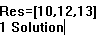
\includegraphics[width=0.48\linewidth]{source/1.png} \\ Пример more\_than}	
	\end{minipage}
	\hfill
	\begin{minipage}[h]{0.48\linewidth}
		\center{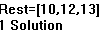
\includegraphics[width=0.48\linewidth]{source/2.png} \\ Пример odd\_list}	
	\end{minipage}
\end{figure}\par

\begin{figure}[h!]
	\begin{minipage}[h]{0.48\linewidth}
		\center{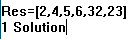
\includegraphics[width=0.48\linewidth]{source/3.png} \\ Пример del\_\/num\_list}	
	\end{minipage}
	\hfill
	\begin{minipage}[h]{0.48\linewidth}
		\center{
\includegraphics[width=0.48\linewidth]{source/4.png} \\ Пример get\_set}	
	\end{minipage}
\end{figure}\par

\newpage
\textbf{Приведем таблицу для cоставления нового списка чисел, больше введенного. }\par
more/than([1],9, Res)\par
Текст процедуры:
\begin{lstlisting}
1:		more_than([], _, []).
2:		more_than([H|T], Num, [H|ResT]):-
				H > Num,
				more_than(T, Num, ResT), !.
3:		more_than([_|T], Num, ResT):-
				more_than(T, Num, ResT).
\end{lstlisting}\par

\begin{table}[]
	\begin{tabular}{|l|l|l|l|}
		\hline
		№ & \begin{tabular}[c]{@{}l@{}}Текущая \\ резольвента - ТР\end{tabular}                         & \begin{tabular}[c]{@{}l@{}}ТЦ, выбираемые правила:\\ сравниваемые термы,\\ подстановка\end{tabular}                                                               & \begin{tabular}[c]{@{}l@{}}Дальнейшие действия\\ с комментариями\end{tabular}        \\ \hline
		1 & more\_than({[}1{]}, 9, Res)                                                                 & ТЦ: more\_than({[}1{]}, 9, Res)                                                                                                                                   & Поиск знания с начала БЗ                                                             \\ \hline
		& more\_than({[}1{]}, 9, Res)                                                                 & \begin{tabular}[c]{@{}l@{}}ПР1:\\ {[}{]} = {[}1{]}\\ \_ = 9\\ {[}{]} = Res\\ Неудача\end{tabular}                                                                 & \begin{tabular}[c]{@{}l@{}}Переход к \\ следующему\\ заголовку БЗ\end{tabular}       \\ \hline
		& more\_than({[}1{]}, 9, Res)                                                                 & \begin{tabular}[c]{@{}l@{}}ПР2:\\ {[}H|T{]} = {[}1{]}\\ Num = 9\\ {[}H1|ResT{]} = Res\\ \\ Успех\\ H = 1\\ T = {[}{]}\\ Num = 9\\ Res = {[}1|ResT{]}\end{tabular} & \begin{tabular}[c]{@{}l@{}}Тело ПР2\\ заменяют цель\\ в резольвенте\end{tabular}     \\ \hline
		2 & \begin{tabular}[c]{@{}l@{}}1 \textgreater 9,\\ more\_than({[}{]}, 9, Res),\\ !\end{tabular} & \begin{tabular}[c]{@{}l@{}}Сравнение:\\ 1 \textgreater 9\\ Неудача\end{tabular}                                                                                   & \begin{tabular}[c]{@{}l@{}}Откат.\\ Переход к следующему\\ заголовку БЗ\end{tabular} \\ \hline
		3 & more\_than({[}1{]}, 9, Res)                                                                 & \begin{tabular}[c]{@{}l@{}}ПР3:\\ {[}\_|T{]} = {[}1{]}\\ Num = 9\\ Res = Res\\ \\ Успех\\ T = {[}{]}\\ Num = 9\\ Res = ResT\end{tabular}                          & \begin{tabular}[c]{@{}l@{}}Тело ПР3 \\ заменяет цель\\ в резольвенте\end{tabular}    \\ \hline
	\end{tabular}
\end{table}

\newpage

\begin{table}[h!]
	\begin{tabular}{|l|l|l|l|}
		\hline
		4 & more\_than({[}{]}, 9, Res) & ТЦ:more\_than({[}{]}, 9, Res)                                                                                      & Поиск знания с начала БЗ                                                                                                                            \\ \hline
		& more\_than({[}{]}, 9, Res) & \begin{tabular}[c]{@{}l@{}}ПР1:\\ {[}{]} = {[}{]}\\ \_ = 9\\ {[}{]} = ResT\\ \\ Успех\\ ResT = {[}{]}\end{tabular} & \begin{tabular}[c]{@{}l@{}}Пустое тело заменяет\\ цель в резольвенте\end{tabular}                                                                   \\ \hline
		& Пусто                      &                                                                                                                    & \begin{tabular}[c]{@{}l@{}}Успех\\ Res = ResT = {[}{]}\\ Откат\end{tabular}                                                                         \\ \hline
		5 & more\_than({[}{]}, 9, Res) & \begin{tabular}[c]{@{}l@{}}ПР2:\\ {[}H|T{]} = {[}{]}\\ Num = 9\\ {[}H|ResT{]} = ResT\\ \\ Неудача\end{tabular}     & \begin{tabular}[c]{@{}l@{}}Переход к следующему\\ заголовку БЗ\end{tabular}                                                                         \\ \hline
		& more\_than({[}{]}, 9, Res) & \begin{tabular}[c]{@{}l@{}}ПР3:\\ {[}\_|T{]} = {[}{]}\\ Num = 9\\ ResT = Res\\ \\ Неудача\end{tabular}             & \begin{tabular}[c]{@{}l@{}}Должен включиться откат,\\ но метки в конце процедур,\\ т.е. других альтернатив нет.\\ \\ Завершение работы\end{tabular} \\ \hline
	\end{tabular}
\end{table}

\textbf{Вывод}\par
Эффективность работы системы может быть достигнута за счет хвостовой
рекурсии и использования отсечения в тех
случаях, где заведомо известна единственность ответа на вопрос.

\newpage

\textbf{Ответы на вопросы}\par

\begin{enumerate} 
	\item Как организуется хвостовая рекурсия в Prolog? 
	
	Хвостовая рекурсия: Для ее осуществления рекурсивный вызов определяемого предиката должен быть последней подцелью в теле рекурсивного правила и к моменту рекурсивного вызова не должно остаться точек возврата (непроверенных альтернатив). 
	
	\item Какое первое состояние резольвенты?
	
	Вопрос. 
	
	\item Каким способом можно разделить список на части, какие, требования к частям?
	
	В Prolog существует более общий способ доступа к элементам списка. Для этого используется метод разбиения списка на начало и остаток. Для этого используется вертикальная черта (|) за последним элементом начала. 
	
	Начало списка -- это группа первых элементов, не менее одного. Остаток списка -- обязательно список (может быть пустой), всегда один. 
	
	\item Как выделить за один шаг первые два подряд идущих элемента списка? Как выделить 1-й и 3-й элемент за один шаг?
	
	Два подряд идущих:
	
	\begin{lstlisting}
		[First, Second|Tail]
	\end{lstlisting}
	
	1-й и 3-й:
	
	\begin{lstlisting}
		[First, _, Third|Tail]
	\end{lstlisting}
	
	\item Как формируется новое состояние резольвенты?
	
	Резольвента - текущая цель, существующая на любой стадии вычислений. Резольвенты порождаются целью и каким-либо правилом или фактом, которые просматриваются последовательно сверху вниз. Если резольвента существует при наиболее общей унификации, она вычисляется. Если пустая резольвента с помощью такой стратегии не найдена, то ответ на вопрос отрицателен.
	
	\item Когда останавливается работа системы? Как это определяется на формальном уровне?
	
	Когда стек пуст. 
	
\end{enumerate}

\end{document}